\chapter {Увоз Боричев}

Боричев увоз (или взвоз), он же, по различным летописным спискам – Зборичев, Биричев, Буричев, Оузборичев, Борищев, Оузборичев, Барнуев, Борнувье, Звозбори уев и так далее. Древняя дорога на Старокиевской горе, соединявшая нижний город Подол с верхним городом. Где был сей Боричев, и почему так назван?

Существует две основные версии его положения. Я сейчас их упрощу. Первая - что увоз Боричев лежал в овраге, где теперь проходит фуникулер или около. Ныне параллельно нижней части фуникулера идет крутая улочка Боричев спуск. 

По другой версии, любимой многими позднейшими историками, Боричев это нынешний Андреевский спуск.

Пора опровергнуть заблуждение относительно Андреевского, и дать обоснование тому, что Боричев это старинная дорога по склону, где нынче маршрут фуникулера, то бишь от Почтовой площади наверх к Михайловскому монастырю, воссозданному в конце 20 века, и зданию МИД. До сих пор сохранились упоминаемые в летописях и старинных грамотах урочища и местности, но сохранился ли сам Боричев?

И что такое Боричев, только ли увоз или ввоз как дорога, соединяющая верх горы с низом, или гораздо большее урочище Боричев? Ведь "увоз" применительно к Боричеву встречается в летописи только один раз. Между тем до сих пор существует перпендикулярная фуникулеру улица Боричев ток, именуемая по урочищу Боричев ток. Быть может летописное урочище Боричев это и есть позднейший Боричев ток?

И в самом ли деле овраг с фуникулером стоит понимать как место летописного увоза Боричева? С одной стороны, глядя на местность, и держа в уме, что где-то тут и был увоз, думаешь - где же еще? С другой стороны имеем мутные сведения, что овраг Боричева был засыпан при устройстве наверху крепости. Закревский приводил слова «старика Вигеля», сетовавшего, что Боричев увоз засыпали, но в воспоминаниях Вигеля я такого не нашел. Как бы ни было, если засыпали, где же тогда на склоне искать сгинувший овраг?

Михаил Максимович в "Обозрении старого Киева"\cite{max} пишет:

\begin{quotation}
Древнейший город Киев начинался там, где Андреевская гора отделяется небольшим оврагом от монастыря Михайловского. Этот овраг есть заглохший след Боричева ввоза. 

[...]

Боричев ввоз проходил с горы там, где теперь Рождественская церковь.

[...]

Некоторые киево-подольские старожилы помнят, что в 1810 году, когда для построения нынешней каменной церкви Рождественской разбирали прежнюю деревянную, построенную 1564 года, то в ее основании найдено было надписание, что она поставлена была на увозе Боричевом
\end{quotation}

Это очень ценные сведения. Накладывая имеющиеся у меня старинные карты на современные (но карты не всегда точны), я не вижу на склоне, именно такого прямого оврага, в котором с 1905 года пролегает линия фуникулера. Да, в протяженности последнего показан некий овраг, но упирающийся в стену Михайловсокого монастыря. 

А вот чуть западнее его на многих картах 19 века есть прорезающий вершину холма 
отрезок оврага. Отрезок лежал между оградой Михайловского монастыря и стеной укрепления, во внутреннем пространстве коего была Васильевская (Трехсвятительская церковь). Ныне на этом отрезке стоит, уже на ровном плато - здание МИД, а далее овраг дотягивался до начала Большой Житомирской улицы.

Васильевская же церковь стояла бы в тылу здания МИД, к северо-западу от него, примерно тут:

50.45723506643367, 30.520857719327125

но по разным картам место несколько "гуляет".

Фрагмент плана 1803 года Меленского:

\begin{center}
\includegraphics[width=\linewidth]{chast-colebanie-osnov/uvoz-borichev/uvoz1803.png}
\end{center}

Зеленый кружочек - Рождественская церковь на Подоле, это еще деревянная, до пожара. Если сопоставление карты верно, то стояла несколько на северо-запад от текущей восстановленной (а ту воссоздали с каменной 1810 года).

Синий кружочек - Васильевская (Трехсвятительсая) церковь наверху, ныне не существует.

Оранжевый овал и около - Михайловский монастырь.

Красный овал - то самое верховье оврага, который врезался в глубину Михайловской площади, это про него Максимович пишет:

\begin{quotation}
где Андреевская гора отделяется небольшим оврагом от монастыря Михайловского. Этот овраг есть заглохший след Боричева ввоза.\end{quotation}

Так что же, можно провести прямую линию между синим и зеленым кружочками и получим летописный увоз Боричев? Он будет лежать параллельно фуникулеру, вблизи, несколько севернее. Примерно на его линии будет и современная улица Боричев спуск, ранее нижняя часть Трехсвятительской, хотя по картам этот нижний отрезок не соединялся с верхом горы, однако нисходил к Подолу начиная от соединения с пепрендикулярной улицей Боричев ток. 

Что же на этой предполагаемой линии сейчас, выше улицы Боричев спуск? Можно ли увидеть на усыпанном старинным кирпичами склоне следы оврага?

Можно, но признаться, когда я лазал там, 
то не искал овраг Боричева увоза, предполагая что он находится по месту оврага с фуникулером. Овраг с фуникулером (не такой ровный как сейчас) есть на карте 1803 года, есть и параллельный овраг (выше улице Боричев спуск, но если учитывать сведения, что исконный Боричев увоз мог быть засыпан (в какой-то мере), мы не можем по местности и картам однозначно вычислить положение Боричева увоза.

Мы знаем точно его верховье, оно погребено ныне под зданием МИД, и мы знаем что Боричев увоз начинался где-то внизу около Рождественской церкви. Вот таковы точные данные.

Выше улицы Боричев спуск по склону ниже здания МИД, помимо старинных кирпичей, находится дренажная система отвода грунтовых вод, и там под землей течет довольно сильный ручей, а вообще местность судя по всему многократно перекапывалась. Но туда мы отправимся чуть позже.

Разберем теперь по крупицам источники, с самого начала. В летописи как сказано? «И седяше Кый на горе, идеже ныне увоз Боричев».

Памятуя, что текст в летописях идет без пробелов между словами, а монахи переписывали всё, как распознавали, предположу, что поначалу в подлиннике могло быть (большими буквами выделено мною): «идеженынеУБОЗБоричев». То есть, «где ныне, убо (стало быть), Зборичев». Зборичев – от сборов, пошлин, ведь где-то внизу (изменение за века прибрежного русла не позволяют вычислить положение пристани в летописное время) находилась пристань, и купцы платили пошлину. Пошлина – слово емкое – платишь за прохождение.

Но это, повторюсь, лишь предположение, 
что слова «увоз» в первом варианте летописного рассказа не было. Просто на горе либо её склоне находилось место под названием Зборичев, где купцы, поднимаясь на гору платили сбор, пошлину. Более того, в дальнейшем летопись упоминает Боричев уже без «увоз» или «взвоз», а просто одним словом – Боричев, в разных его вариантах.

Но вернемся ко классическому толкованию, когда слово «увоз» всё же присутствует. К тому же всё равно нужна дорога, путь соединения между верхом и низом.

Путаница первая. В старину словом «увоз»
обозначали не только дорогу, соединявшую низ и верх горы, но также переправу либо перевоз. 

Если около нынешней Почтовой площади была пристань, то и переправа. Это согласуется с версией, что Кий был не князем, но перевозчиком. Нестор перед опровержением пишет: «не сведущие рекоша яко кий есть перевозник был. от киева бо бяше перевоз тогда с оной стороны днепра тем глаголаху на перевоз на киев».

Перевоз, переправа, увоз. Поэтому и увоз Боричев?

Между тем, в некоторых списках летописи вместо «увоз» стоит «взвоз». Взвоз – это подъем от чего-либо. Тоже вариант. Взвоз Боричев, Зборичев – дорога наверх, по ходу которой с купцов брали пошлину. Зборы, сборы, боры – от брать. Биричев – от того же, в одной грамоте сказано, «биривали» в значении «брали». Хотя известно и слово «бирич» – глашатай, объявлявший в народе княжеские приказы.

Но могла ли дорога в овраге между нынешней Почтовой площадью и верхом горы, дорога в окрестностях фуникулера, служить путем для перемещения грузов? Величина уклона там составляет 18-20 градусов. Возникает вопрос о том, как пользовались дорогой. Вот пристань, к ней прибывают корабли с грузами. Грузы с пристани доставлялись наверх вручную? Или купцы нанимали возы?

Летом 2013 года я катался в том краю на велике и хотел съехать по улице Боричев спуск, частично параллельной фуникулеру. Пришлось резко тормозить и спешиться, ибо живым я бы до конца улицы не добрался – слишком круто.

Тогда я задумался. Если летописный увоз Боричев проходил где-то здесь, как оттуда съезжали и поднимались на возах? Продолжая рассуждать в таком духе, я поначалу пришел к мысли, что дорога наверх шла не прямо, а изгибами взбиралась по террасам холма.  Таковые есть поныне, но когда они возникли?

На крутизну нынешнего подъема по ходу фуникулера указывают и сторонники версии об Андреевском спуске. Мол, непригодно для сообщения. Пешком еще можно, а вот грузы, да на возах – невозможно. 

Но мы знаем, что раньше увоз Боричев оврагом входил, постепенно повышаясь, вглубь нынешней Михайловской площади, как бы прорезая ее. Следовательно в том месте у оврага был меньший угол наклона, что у склона. Каков же был угол наклона у остальной части Боричева увоза? Тоже меньшим? 

Или дорога таки петляла по терассам, чтобы потом свернуть на место МИДа? Долговато, хотя дорога могла состоять, на разных своих участках, из террас и из прямого подъема.

К тому же, как я покажу далее в этой книге, в Киеве поныне сохраняется еще две старинные дороги в оврагах - одна на Замковой горе, другая вдоль Иорданского кладбища. В оврагах, чье дно имеет меньший угол наклона, чем у склона, таким образом по оврагу лечче преодолевать высоту.

Давайте познакомимся с местностью ближе.

Нас интересует северо-восточный склон Старокиевской горы, уступами нисходящий к Подолу в сторону Днепра. На самом верху, у края холма, на Михайловской площади, расположены здание МИДа и Михайловский собор. Между ними пространство, и около кромки холма – верхняя станция фуникулера. Оттуда по прямой, в овраге со спрямленными берегами, фуникулер спускается к своей нижней станции, на Почтовую площадь Подола.

На пригорке, где расположился МИД, была верхняя часть оврага, и там на его северном берегу Владимир поставил, "вне двора теремна", идолов, в том числе идола Перуна, коего во время массового крещения киевляин по приказу Владимира же и низвергнули. На том месте построили церковь святого Василия, по христианскому имени князя Владимира. В 17 веке на ее остатках Петром Могилой была поставлена новая, Трехсвятительская, затем она горела, восстановлена в 1783 и разрушена в 1935-36 годах. На картах 19 века название то Трехсвятительская, то Васильевская.

Ниже МИДа и Михайловского монастыря лежит терраса с теперь прогулочной дорогой, идущей сначала по Владимирской горке (под монастырем) и дальше в сторону Андреевской церкви, огибая её с востока и севера, дабы затем соединиться с Андреевским спуском. Дорога проходит под фуникулером, немного ниже верхней его платформы. Когда появились эти террасы – история умалчивает.

Еще ниже по склону – терраса с улицей Боричев Ток, названной так по имени местности. От Боричева Тока круто вниз, к улице Сагайдачного и Почтовой площади, перпендикулярно отходит короткая улица Боричев спуск.

До 1869 года отдельной улицы Боричев спуск не было. Она являлась частью продолженной наверху горы Трехсвятительской улицы, не соединяясь с нею. После 1869 сей отрезок получил самостоятельность и название «Боричева ввоза».

Теперь карта. Я сделал прорисовку по аэрофотоснимку 1943 года. С тех пор расположение улиц не изменилось.
\vspace*{\fill}
\begin{center}
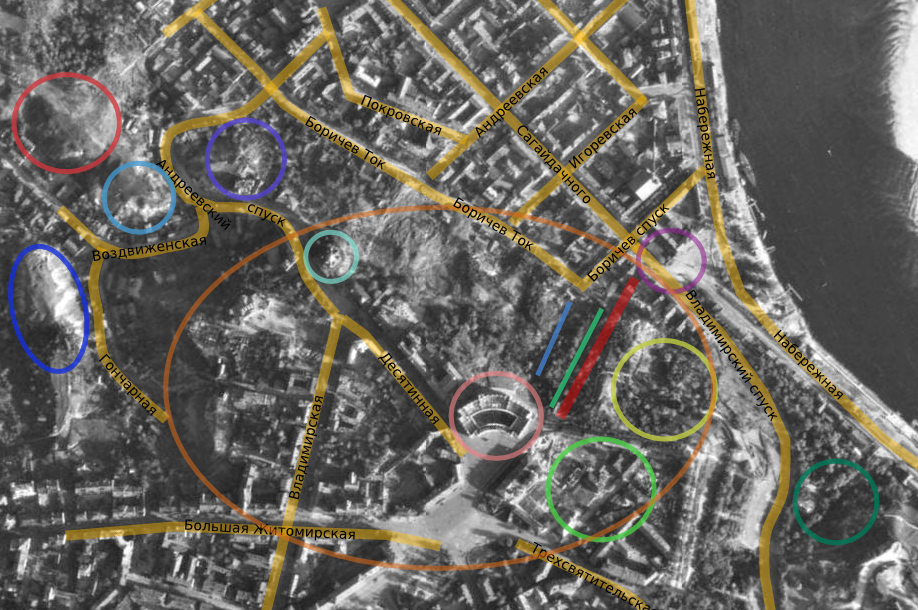
\includegraphics[width=\linewidth]{chast-colebanie-osnov/uvoz-borichev/bor-karta.jpg}
\end{center}
\vspace*{\fill}
\newpage

Линии:

\begin{itemize}
\item Красная – фуникулер, проложенный в ровненьком овраге.

\item Зеленая рядом с ним – северо-западная сторона этого оврага, где видны остатки некоего вала. Вал сей продолжается почти до самого низа.

\item Голубая – чуть в отдалении от вала (снова на северо-запад) по склону сочился ручей, вероятно именно он извстен в прошлом как «Боричев поток» – отсюда кажется и название нижележащей местности Боричев ток. 

Сейчас ручей перехвачен по склону дренажной системой, вода его весьма чиста, во всяком случае без запаха химии, а течение довольно бойкое.
\end{itemize}

Кружки:

\begin{itemize}
\item Розовый – здание МИД. Довлеет над окрестностями.

\item Бордовый – Почтовая площадь.

\item Желтый – Владимирская горка.

\item Салатовый – Михайловский монастырь.

\item Зеленый – Хрещатое (Крещатое) урочище, там где лестница к памятнику Магдебургскому праву. Прежде там был съезд к старой набережной дороге.

\item Бирюзовый – Андреевская церковь.

\item Фиолетовый – гора Уздыхальница.

\item Голубой – гора Клинец.

\item Красный – гора Замковая.

\item Синий – гора Детинка.

\item Оранжевый – Старокиевская гора, как можно судить, именуемая в некоторых списках Киевицей. Само название Старокиевская в давних источниках отсутствует, это скорее современный научный термин.
\end{itemize}

Давайте подробно пройдемся по всей местности и обсудим её. Посмотрим, где и как она находит отражение в летописях, старинных грамотах, на давних картах и фотографиях. 

\newpage

Вот сам фуникулер. Снято как раз с той дороги, что по террасе идет от Владимирской горки (под Михайловским монастырем) и далее, огибая склон, в сторону Андреевской церкви. Отметим вал слева. 
\vspace*{\fill}
\begin{center}
\includegraphics[width=\linewidth]{chast-colebanie-osnov/uvoz-borichev/\myimgprefix IMG_20131013_145318.jpg}
\end{center}
\vspace*{\fill}
Если на него встать и посмотреть вдоль, можно заметить, что проложен он по ровной линии. От вала налево начинается ложбина, где стекал Боричев поток и которая возможно и есть исходный увоз Боричев, ибо это продолжение верхней части оврага (части что прорез\'ала Михайловскую площадт), если он нисходил по прямой линии.

Противоположный берег оврага с фуникулером – намного выше, чем вал. Откос этого берега и следы постепенного оползания почвы дают основания полагать, что некогда овраг в тех пределах был шире, да и на карте 1803 года овраг широк.

Местность справа считается нынче Владимирской горкой.

Внизу, у Почтовой площади, видна арка нижней станции фуникулера, до которой около 140 метров. А до верхней – всего тридцать. Непосредственно слева за кадром находится будка тяговой подстанции. Ее стены служат туалетом для киевлян и гостей столицы, равно как и все окрестности.

\newpage

Теперь пройдем несколько шагов в сторону и поглядим наверх:

\begin{center}
\includegraphics[width=\linewidth]{chast-colebanie-osnov/uvoz-borichev/\myimgprefix borichev-IMG_20131013_145300.jpg}
\end{center}

Вот так над дорогой (напомню, что мы стоим на террасе) проложен фуникулер. Впереди, на пригорке, видим его верхнюю станцию. За нею правее будет здание МИД, а слева на том же уровне – Михайловский монастырь.

И несколько правее сего места и был отрезок оврага Боричева увоза, над коим (над отрезком), на месте коего, непосредственно стоит здание МИД. 

На Плане Ушакова 1695 года на том месте таки овраг, подписанный "боярак", и ниже некое сооружение в нисходящем к террасе овраге. 

Скорее всего, сие известная в 18 веке «Михайловская калитка» к нижележащему Михайловскому спуску, что сходил примерно к церкви Рождества, а значит лежал там же, где и увоз Боричев. Одно время Михайловским спуском вроде бы именовался и нынешний Владимирский спуск, но прежде того, в грамоте Сигизмунда I, разрешающей восстановление Михайловского Златоверхого монастыря, от 15 марта 1523 года, границы землевладения оного определяются так:

\begin{quotation}
и земли к тому манастырю мает держати по даному, как перед тым бывало, по самый вал, и по Лядскии ворота, и по Евсийкову долину, по старую дорогу, по Михайловский ввоз.
\end{quotation} 

И вот упоминаются старая дорога и Михайловский ввоз как соседние части границы. "Владимирского спуска" тогда не было, был спуск в урочище Крещатик, внизу соединявшийся со старой набережной дорогой. 
И была дорога к Михайловскому монастырю, примерно где теперь улица Михайловская. 

Четкая привязка именования Михайловского ввоза к дороге наверх от Рождественской церкви к "бояраку" около Михайловского монастыря будет в главе про Почайну, не хочу здесь повторять текст. Можем с большой степенью вероятности отождествить старинный Михайловский ввоз с местом летописного Боричева увоза, а его с большой вероятностью представить параллельно линии фуникулера, немного севернее его, там где сейчас дренажка ручья, где я полагаю Боричев поток. Примечательно, что многие дороги в Киеве прежде проходили именно в оврагах с ручьями. Это и Старый Никольский ввоз, и вот спуск в урочище Хрещатик, получается и увоз Боричев тоже.

Вид со стороны Днепра, боярак посередке, слева, в общем, Михайловский монастырь, к нему тогда примыкал еще Свято-софиевский девичий:

\begin{center}
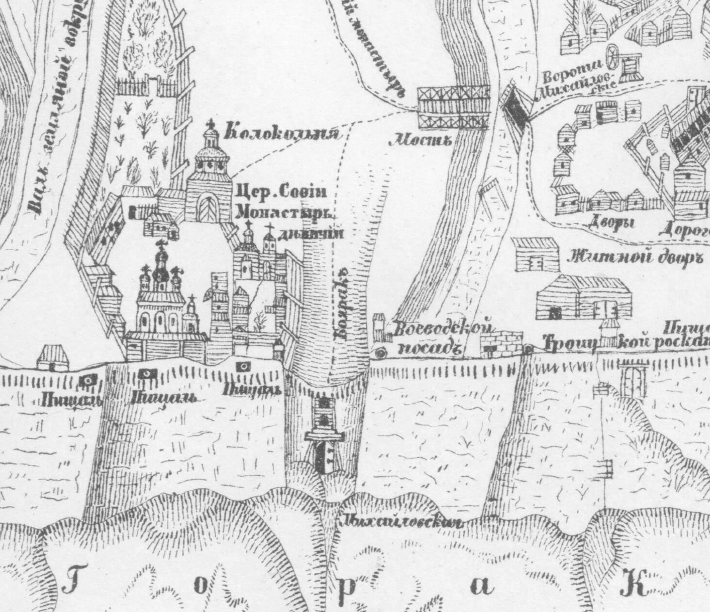
\includegraphics[width=\linewidth]{chast-colebanie-osnov/uvoz-borichev/1695-borichev.png}
\\
\textit{Фрагмент плана Ушакова.}
\end{center}

Жаль что по карте нельзя понять, как же продолжался сей овраг ниже, в сторону или праямо, да и топографическая точность плана оставляет желать много, много лучшего.

Уточнение – во время составления плана, к буераку выходил не Михайловский, но соседний Софиевский монастырь (не путать с Софией, она юго-западнее), переведенный затем на Кирилловские высоты под именем Богословского, где ныне Богуславский спуск.

Однако по этой карте и по карте 1803 года боярак, читай - верховье увоза Боричева - дотягивало до современной Большой Житомирской улицы. Это примерно 250 метров от северо-восточного угла здания МИД. Чуть больше - около 300 метров - от подольской церкви Рождества, хотя мы не знаем, где именно внизу была граница увоза. Но в нынешнюю Михайловскую площадь вписывалась чуть ли не половина всей длины увоза. Такая длина обусловлена "сбрасыванием" высоты, малым углом наклона. Имел ли Боричев увоз на всей своей протяженности одинаковый уклон? Думаю да, и именно малым углом наклона всего увоза и обусловлена дальность буерака вглубь площади, иначе буерак был бы значительно короче. Чем длиннее, чем меньше угол наклона.

Таким образом склон горы был круче, нежели дно оврага, который – как ясно из карты – вдавался глубоко в склон относительно его края. 

Чем больше угол наклона, тем короче дорога. Боярак удлинял дорогу и сбавлял угол наклона. 

Эта удивительная дорога в ущелье делала возможным подъем по ней относительно легким делом. Потому что иначе, 20 градусов подъема нынешнего склона там где фуникулер – это и пешком осилить тяжело, не говоря уже о ручной переноске грузов.

%КАКОЙ БЛИН СОФИЕВСКИЙ?
%Любопытно, что Софиевский монастырь был перенесен в место, где поныне сохранилась, за Иорданским переулком, старинная дорога на Лукьяновку, которая в точности повторяет прежний Боричев, плавно вписываясь внутрь холма по желобу длинного оврага.

«Боярак» в верховьях Боричева просматривается на картах, после плана Ушакова, довольно долго. От крепостной стены у северо-западного берега оврага, к противоположному берегу с Михайловским монастырем (на уровне его юго-западного края) через овраг был перекинут мост, заметный еще на плане 1812 года. Спустя несколько десятилетий там уже ровное место.

По старинным фотографиям хорошо видно, как только за последние десятилетия 19 века и начало 20-го менялся склон, как в одних местах его крутизна сглаживалась террасами, а в других – напротив, с течением времени и земляных работ, увеличивалась. Представьте, сколь исказился рельеф с летописных времен! Петру I нужна наверху крепость? Склоны делаются обывистей, удобные подходы уничтожаются, овраги засыпаются, гора становится частью крепости, а склон естественным продолжением валов по его краю. Попробуй заберись! 

Затем эпоха строгости чуть смягчается, фортификационные сооружения в центре города мешают. Валы сравниваются, крепостные стены исчезают. Появляется необходимость в соединении Подола около Почтовой площади с верхним городом. Человек снова трудится, облегчает себе дорогу.

Вот пример. Два снимка, вид на фуникулер – или, как тогда говорили, Михайловский подъем – с Владимирской горки. 

На первом склон под церковью Василия, непосредственно справа от верхней площадки фуникулера, обрывист и дик. У опор под рельсами видны строительные леса либо дополнительные подпорки. Вдоль тропы слева – косой забор.

\begin{center}
\includegraphics[width=\linewidth]{chast-colebanie-osnov/uvoz-borichev/\myimgprefix fun-13.jpg}
\end{center}

И далее снимок, сделанный позже. Заметно, что участок под церковью сделан более пологим за счет уступов. За ним, в сторону Андреевской церкви, угол наклона тоже уменьшен – насыпали землю, она не заросла еще травой. Дальше снова дорожки по террасам на месте некогда сплошного склона. Слева же дорожка проходит иначе, и снабжена оградкой, а за нею ровненьким забором.

\begin{center}
\includegraphics[width=\linewidth]{chast-colebanie-osnov/uvoz-borichev/\myimgprefix mihpod04.jpg}
\end{center}
